\documentclass{beamer}

\usepackage[utf8]{inputenc}
\usepackage{gnuplot-lua-tikz}
\usepackage{tikz}
\usetikzlibrary{positioning}

\title{Using binary decision diagrams to determine program equivalence in a superoptimizer}
\author{Jesper Särnesjö}
\date{}

\begin{document}

\begin{frame}
\titlepage
\end{frame}

\begin{frame}
\begin{figure}
\include{so_program_length_1}
\end{figure}
\end{frame}

\begin{frame}
\begin{figure}
\include{so_program_length_2}
\end{figure}
\end{frame}

\begin{frame}
\begin{figure}
\include{so_program_length_3}
\end{figure}
\end{frame}

\begin{frame}
\begin{figure}
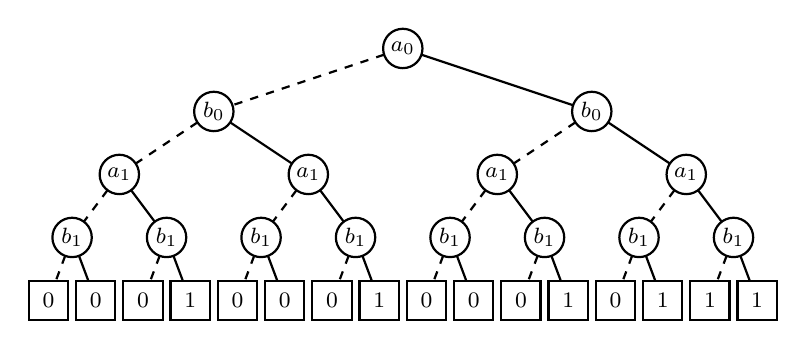
\begin{tikzpicture}
[every node/.style={draw=black,thick,minimum size=5mm,inner sep=0mm,outer sep=0mm,font=\footnotesize},
 var/.style={circle},
 val/.style={rectangle},
 thick]
\node[var] (a0)                                            {$a_0$};
\node[var] (b0A) [on grid,below  left=8mm and 24mm of a0]  {$b_0$};
\node[var] (b0B) [on grid,below right=8mm and 24mm of a0]  {$b_0$};
\node[var] (a1A) [on grid,below  left=8mm and 12mm of b0A] {$a_1$};
\node[var] (a1B) [on grid,below right=8mm and 12mm of b0A] {$a_1$};
\node[var] (a1C) [on grid,below  left=8mm and 12mm of b0B] {$a_1$};
\node[var] (a1D) [on grid,below right=8mm and 12mm of b0B] {$a_1$};
\node[var] (b1A) [on grid,below  left=8mm and  6mm of a1A] {$b_1$};
\node[var] (b1B) [on grid,below right=8mm and  6mm of a1A] {$b_1$};
\node[var] (b1C) [on grid,below  left=8mm and  6mm of a1B] {$b_1$};
\node[var] (b1D) [on grid,below right=8mm and  6mm of a1B] {$b_1$};
\node[var] (b1E) [on grid,below  left=8mm and  6mm of a1C] {$b_1$};
\node[var] (b1F) [on grid,below right=8mm and  6mm of a1C] {$b_1$};
\node[var] (b1G) [on grid,below  left=8mm and  6mm of a1D] {$b_1$};
\node[var] (b1H) [on grid,below right=8mm and  6mm of a1D] {$b_1$};
\node[val] (tA)  [on grid,below  left=8mm and  3mm of b1A] {0};
\node[val] (tB)  [on grid,below right=8mm and  3mm of b1A] {0};
\node[val] (tC)  [on grid,below  left=8mm and  3mm of b1B] {0};
\node[val] (tD)  [on grid,below right=8mm and  3mm of b1B] {1};
\node[val] (tE)  [on grid,below  left=8mm and  3mm of b1C] {0};
\node[val] (tF)  [on grid,below right=8mm and  3mm of b1C] {0};
\node[val] (tG)  [on grid,below  left=8mm and  3mm of b1D] {0};
\node[val] (tH)  [on grid,below right=8mm and  3mm of b1D] {1};
\node[val] (tI)  [on grid,below  left=8mm and  3mm of b1E] {0};
\node[val] (tJ)  [on grid,below right=8mm and  3mm of b1E] {0};
\node[val] (tK)  [on grid,below  left=8mm and  3mm of b1F] {0};
\node[val] (tL)  [on grid,below right=8mm and  3mm of b1F] {1};
\node[val] (tM)  [on grid,below  left=8mm and  3mm of b1G] {0};
\node[val] (tN)  [on grid,below right=8mm and  3mm of b1G] {1};
\node[val] (tO)  [on grid,below  left=8mm and  3mm of b1H] {1};
\node[val] (tP)  [on grid,below right=8mm and  3mm of b1H] {1};
\path[dashed] (a0)  edge (b0A);
\path         (a0)  edge (b0B);
\path[dashed] (b0A) edge (a1A);
\path         (b0A) edge (a1B);
\path[dashed] (b0B) edge (a1C);
\path         (b0B) edge (a1D);
\path[dashed] (a1A) edge (b1A);
\path         (a1A) edge (b1B);
\path[dashed] (a1B) edge (b1C);
\path         (a1B) edge (b1D);
\path[dashed] (a1C) edge (b1E);
\path         (a1C) edge (b1F);
\path[dashed] (a1D) edge (b1G);
\path         (a1D) edge (b1H);
\path[dashed] (b1A) edge (tA);
\path         (b1A) edge (tB);
\path[dashed] (b1B) edge (tC);
\path         (b1B) edge (tD);
\path[dashed] (b1C) edge (tE);
\path         (b1C) edge (tF);
\path[dashed] (b1D) edge (tG);
\path         (b1D) edge (tH);
\path[dashed] (b1E) edge (tI);
\path         (b1E) edge (tJ);
\path[dashed] (b1F) edge (tK);
\path         (b1F) edge (tL);
\path[dashed] (b1G) edge (tM);
\path         (b1G) edge (tN);
\path[dashed] (b1H) edge (tO);
\path         (b1H) edge (tP);
\end{tikzpicture}

\end{figure}
\end{frame}

\begin{frame}
\begin{figure}
\include{bdd_c1_2}
\end{figure}
\end{frame}

\begin{frame}
\begin{figure}
\include{bdd_c1_3}
\end{figure}
\end{frame}

\begin{frame}
\begin{figure}
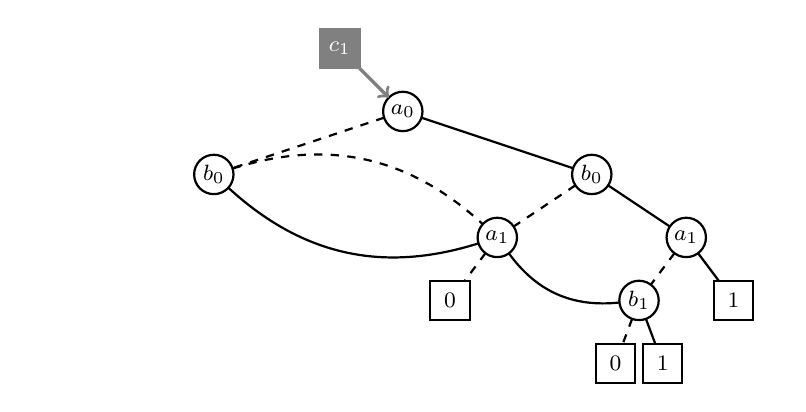
\begin{tikzpicture}
[every node/.style={draw=black,thick,minimum size=5mm,inner sep=0mm,outer sep=0mm,font=\footnotesize},
 var/.style={circle},
 val/.style={rectangle},
 ref/.style={rectangle,white,draw=gray,fill=gray},
 hl/.style={rectangle,draw=red,minimum size=7mm},
 thick]
\node[var] (a0)                                            {$a_0$};
\node[var] (b0A) [on grid,below  left=8mm and 24mm of a0]  {$b_0$};
\node[var] (b0B) [on grid,below right=8mm and 24mm of a0]  {$b_0$};
\node[var] (a1C) [on grid,below  left=8mm and 12mm of b0B] {$a_1$};
\node[var] (a1D) [on grid,below right=8mm and 12mm of b0B] {$a_1$};
\node[val] (b1E) [on grid,below  left=8mm and  6mm of a1C] {0};
\node[var] (b1G) [on grid,below  left=8mm and  6mm of a1D] {$b_1$};
\node[val] (b1H) [on grid,below right=8mm and  6mm of a1D] {1};
\node[val] (tM)  [on grid,below  left=8mm and  3mm of b1G] {0};
\node[val] (tN)  [on grid,below right=8mm and  3mm of b1G] {1};
\path[dashed]           (a0)  edge (b0A);
\path                   (a0)  edge (b0B);
\path[bend left,dashed] (b0A) edge (a1C);
\path[bend right]       (b0A) edge (a1C);
\path[dashed]           (b0B) edge (a1C);
\path                   (b0B) edge (a1D);
\path[dashed]           (a1C) edge (b1E);
\path[bend right]       (a1C) edge (b1G);
\path[dashed]           (a1D) edge (b1G);
\path                   (a1D) edge (b1H);
\path[dashed]           (b1G) edge (tM);
\path                   (b1G) edge (tN);

\node[ref] (Rc1) [on grid,above left=8mm and 8mm of a0] {$c_1$};
\path[->,gray,very thick] (Rc1) edge (a0);

% included on every picture to make sure a0 stays centered
\node[draw=white] (xA) [on grid,below  left=32mm and 45mm of a0] {};
\node[draw=white] (xb) [on grid,below right=32mm and 45mm of a0] {};
\end{tikzpicture}

\end{figure}
\end{frame}

\begin{frame}
\begin{figure}
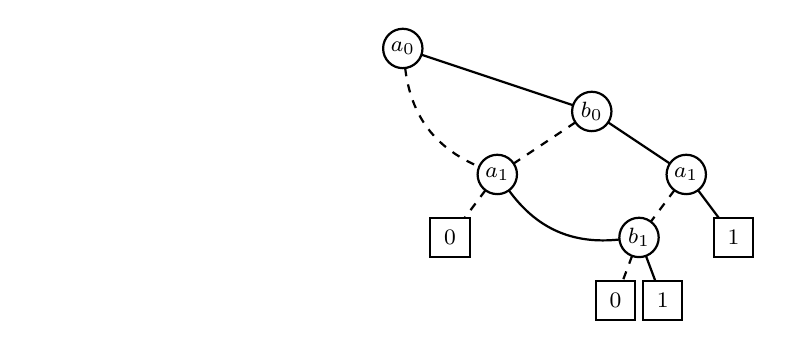
\begin{tikzpicture}
[every node/.style={draw=black,thick,minimum size=5mm,inner sep=0mm,outer sep=0mm,font=\footnotesize},
 var/.style={circle},
 val/.style={rectangle},
 hl/.style={rectangle,draw=red,minimum size=7mm},
 thick]
\node[var] (a0)                                            {$a_0$};
\node[var] (b0B) [on grid,below right=8mm and 24mm of a0]  {$b_0$};
\node[var] (a1C) [on grid,below  left=8mm and 12mm of b0B] {$a_1$};
\node[var] (a1D) [on grid,below right=8mm and 12mm of b0B] {$a_1$};
\node[val] (b1E) [on grid,below  left=8mm and  6mm of a1C] {0};
\node[var] (b1G) [on grid,below  left=8mm and  6mm of a1D] {$b_1$};
\node[val] (b1H) [on grid,below right=8mm and  6mm of a1D] {1};
\node[val] (tM)  [on grid,below  left=8mm and  3mm of b1G] {0};
\node[val] (tN)  [on grid,below right=8mm and  3mm of b1G] {1};
\path[bend right,dashed] (a0)  edge (a1C);
\path                    (a0)  edge (b0B);
\path[dashed]            (b0B) edge (a1C);
\path                    (b0B) edge (a1D);
\path[dashed]            (a1C) edge (b1E);
\path[bend right]        (a1C) edge (b1G);
\path[dashed]            (a1D) edge (b1G);
\path                    (a1D) edge (b1H);
\path[dashed]            (b1G) edge (tM);
\path                    (b1G) edge (tN);

% included on every picture to make sure a0 stays centered
\node[draw=white] (xA) [on grid,below  left=32mm and 45mm of a0] {};
\node[draw=white] (xb) [on grid,below right=32mm and 45mm of a0] {};
\end{tikzpicture}

\end{figure}
\end{frame}

\begin{frame}
\begin{figure}
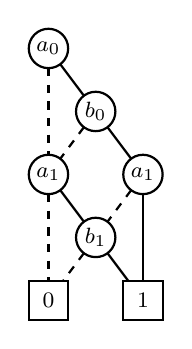
\begin{tikzpicture}
[every node/.style={draw=black,thick,minimum size=5mm,inner sep=0mm,outer sep=0mm,font=\footnotesize},
 var/.style={circle},
 val/.style={rectangle},
 thick]
\node[var] (a0)                                           {$a_0$};
\node[var] (b0B) [on grid,below right=8mm and 6mm of a0]  {$b_0$};
\node[var] (a1C) [on grid,below  left=8mm and 6mm of b0B] {$a_1$};
\node[var] (a1D) [on grid,below right=8mm and 6mm of b0B] {$a_1$};
\node[var] (b1G) [on grid,below  left=8mm and 6mm of a1D] {$b_1$};
\node[val] (tM)  [on grid,below  left=8mm and 6mm of b1G] {0};
\node[val] (tN)  [on grid,below right=8mm and 6mm of b1G] {1};
\path[dashed] (a0)  edge (a1C);
\path         (a0)  edge (b0B);
\path[dashed] (b0B) edge (a1C);
\path         (b0B) edge (a1D);
\path[dashed] (a1C) edge (tM);
\path         (a1C) edge (b1G);
\path[dashed] (a1D) edge (b1G);
\path         (a1D) edge (tN);
\path[dashed] (b1G) edge (tM);
\path         (b1G) edge (tN);
\end{tikzpicture}

\end{figure}
\end{frame}

\end{document}
